\documentclass{article}
\usepackage[utf8]{inputenc}

\title{Invariance to atom permutations - Bag of Histogram Bonds}
\author{Viviana Petrescu }
\date{May 2015}

\usepackage{natbib}
\usepackage{graphicx}

\begin{document}

\maketitle

\section{Abstract}
The high computational cost of quantum chemistry calculations have prompted the use of less expensive machine learning methods for predicting molecular properties in chemical compound space.
Finding good feature representations for molecules is hard, in part because of the graph-like structure geometry of the molecules that need to be represented as high dimensional vectors. The desired properties of a descriptor are invariance to rotation and translation of the molecule and invariance with respect to the permutation of atom indexes.
In this work we present a new histogram based descriptor which tries to overcome the above problems. While there are other descriptors which overcome the translation and rotation invariance using Coloumb repulsion information, the main property of the proposed descriptor is its invariance to atom indexing. Moreover, its dimensionality is independent of the size of the molecules and it varies with the number of \textit{distinct} atom types in the dataset.
We evaluate its predictive performance on two datasets (with approx 7k molecules each) which gives close to state of the art predictions of atomization energy using neural networks. 

\section{Introduction}
The discovery of new molecular materials in chemistry has the potential of solving many of the problems we face today.
Having a system which predicts both accurately and at a small computational cost the properties of new materials is highly desirable and has applications ranging from novel drugs discovery, water purification to efficient materials for high energy transmission and storage\cite{cleanenergy}.

Any molecular property can be derived numerically by solving Schröedinger's equation, a setup which is computationally feasible only for small systems. Many approximation algorithms exists which have polynomial complexity in the number of atoms. However, they can also be prohibitive in practice, since predicting one property can take hours or even days for certain system sizes.
If instead, the properties of molecules can be estimated using trained machine learning models, the prediction for a new property of a new unseen molecule can take a couple of milliseconds. To date, kernel ridge regression, Gaussian processes and neural networks have been successfully applied to predicting properties of molecules such as atomization energy, averaged molecular polarizability, HOMO and LUMO eigenvalues or ionization potentials \citep{assessment}.

Machine Learning models are as powerful as the feature descriptors used are. There is a long history of molecular descriptors \cite{todeschini2000handbook} that aim at encoding the information in molecules in a discriminative manner. While some of them require extensive domain knowledge, recent approaches \cite{initialcoloumb} use only the 3D position of atoms and their nuclear charges for describing a molecule.

In the following section we describe two popular descriptors based on Coloumb interactions and we introduce our novel descriptor. In section 3 we describe the datasets on which we evaluate the performance of our model and discuss our experimental results. We summarize the contributions of this work in the last section.

\section{Molecular descriptors}

To better describe the datasets and the properties of the molecular descriptors, we introduce the notations below:
\begin{itemize}
\item $N$ maximum number of atoms in a molecule (present in our dataset)
\item $N_i$ maximum number of atoms of type $i$ that constitute a molecule, where $i$ $\in \{H, O, C, N, S\}$
\item $N_A$ number of different atom types in the dataset
\item $D_{max}$ maximum distance between two pairs of atoms in a molecule
\item $q$ quantization level, a number in $(0,1]$ which defines the coarseness of the histogram of distances
\end{itemize}
The desired properties of a molecular descriptor are
\begin{itemize}
 \item invariance to atom permutation
 \item invariance to translation and rotation
\end{itemize}

\subsection{Coloumb Matrix}
The Coloumb matrix\citep{initialcoloumb} $M^{NxN}$ is a descriptor based on  Coloumb interaction terms between pairs of atoms. These are the terms that appear in equation.//TODO

\[M(i,j) = \left\{
  \begin{array}{lr}
    0.5*Z_i^{2.4} & if i = j\\
    Z_i * Z_j / |R_i - R_j| & otherwise
  \end{array}
\right.
\]

The size of the Coloumb descriptor is given by $\frac{N*(N - 1)}{2}$ if we take into account the symmetry of the matrix.

While the Coloumb matrix solves the translation and rotation invariance, the permutation of atom indexes is solved using variants of the descriptor called Sorted Coloumb Matrix or Randomly Sorted Coloumb Matrices.  Sorted Coloumb Matrix uses the ordering of the atoms obtained by sorting the rows according to their norm. Unlike the simple Coloumb matrix, any molecule has a unique Sorted Coloumb matrix representation.
In practice,  the norm of the rows of a matrix are very close to each other and therefore susceptible to small noise which can lead to a different ordering of the atoms for a molecule. Randomly Sorted Coloumb matrices have been introduced to cope with this issue by adding a small Gaussian noise to every row in the Coloumb Matrix and sort according to the new noisy norm value.

\subsection{Bag Of Bonds}
The descriptor which gives state of the art results in predicting atomization energy is called Bag of Bonds (BoB), whose name was inspired from natural language processing bag of words. In BoB, every bag contains all the pairwise interactions between two types of atoms (the types can be identical). Invariance to indexing of the atoms is obtained by sorting the values inside each bag according to their magnitude.
One possible cause for the robustness of the descriptor is the fact that one bag is responsible for certain types of bonds only.
Its dimensionality  is given by $\sum_i \frac{N_i*(N_i-1)}{2} + \sum_{i,j, i!=j} N_i*N_j	$ .
The first term counts the number of bonds between atoms of the same type and the second term counts the number of bonds between different atom types.

\subsection{Bag of Bonds Histogram}
We propose a new descriptor Bag of Bonds Histogram(BoBH), whose size is not dependent on the number of atoms in the molecules. Similarly with BoB, every bag  encodes information about certain types of bonds. Unlike BoB, where the elements in every bag are sorted according to their magnitude, in BoBH case every bag is a histogram of quantized distances. The size of the bag histogram is given by the maximum distance between two pairs of atoms (pertaining to that bag type). The quantization level of the distances varies between bag types and we experimentally found that a quantization level of 0.2 or 0.25 perform well in practice, but this will vary for different datasets.

Thus, for a given molecule, the BoBH descriptor will encode
\begin{itemize}
\item 
for every different atom type present in the dataset, count how many times it appears in the molecule
\item  
for every pair of atoms of certain type, count how many times the distance between them is in a given quantization interval 
\end{itemize}

An example is given in Fig \ref{fig:BoBH} for a molecule $C_{4}H_{2}O$ with a quantization level of $q=1$. In this example, first the bags containing H were concatenated, then the ones containing C and in the end the ones containing O, resulting in a descriptor of size 21. In general, the size of the descriptor is given by $NA + \sum_i \frac{N_A*(N_A+1)}{2} *\frac{D_{max}}{q} $ 

\begin{figure}[h!]

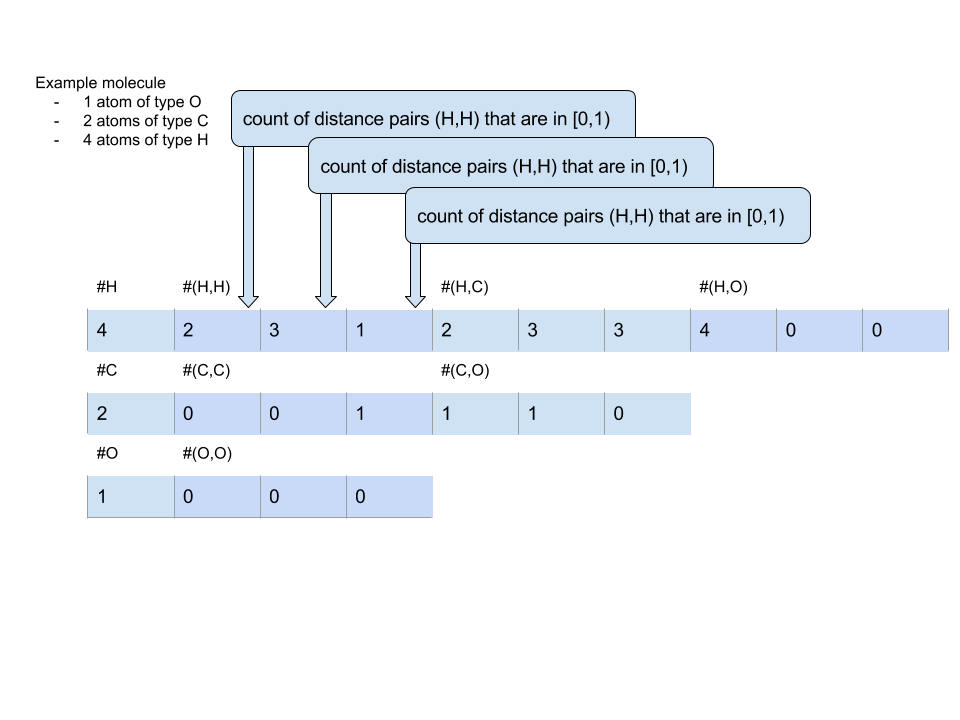
\includegraphics[scale=0.4]{HistogramOfDistances.png}
\caption{Bag of Quantised Bonds.
Sample computation of Bag of Bonds Histogram for $C_2H_4O$ for a dataset which contains only atoms of type O, C and H. If the maximum distance between any two atoms in our dataset is 3, the size of the BoBH descriptor with quantization level  1 is 21, as shown above. The first entry encodes the number of H atoms, 4. The following 3 elements encode the number of (H,H) distances that fall in the interval [0,1), [1,2) and [2,3).
//TODO -> add cool picture showin an actual histogram
}
\label{fig:BoBH}
\end{figure}


To sum up, all descriptors achieve translation and rotation invariance through the use of
distances between atoms instead of the actual 3D positions. Sorted Coloumb and Randomly Sorted Coloumb achieve invariance to index permutation by sorting the rows of the matrix according to their norm. Bag of Bonds sorts the bonds inside each bag and Bag of Bonds Histogram quantizes the distances into bins to bypass the sorting step present in other descriptors.

%//TODO maybe remove this BagOfBonds gives state of the art result on the GDB dataset
%but it is harder to retrieve the actual molecule from the descriptor.
%\begin{tabular}{ l l l l }
%& Dimensionality & Invariance  & \\ 
%&  & to rotation and translation & to permutation \\ 
% Coloumb Matrix& 1& 2 & 3 \\
% Bag Of Bonds & 1& 2 & 3 \\
% Histogram Of Quantised Distances &1 & 2 & 3  \\
%\end{tabular}


\subsection{State of the art results}
The result of \cite{montavon2012learning} were the first ones using neural networks...bla bla


\section{Experiments}
The data was normalised to have values between 0 and 1. Unlike standardization,
we believe this helps more the network to learn, since it keeps the values in the same regime as the initialization fo the weights and biases.
We experimented with various quantization level, between 1 to 0.20.
We used Whetlab tool for finding best network arhitecture. Unlike grid search, the tool uses gaussian processes to find the best parameters for a model.
Since for us ReLU activation seemed to perform better, possibly also due to its inherently nature of generating sparse representations and for the inherently sparse nature of our feature descriptor.

\subsection{Datasets description}
Our currated dataset GDB-7 consists of 7122 molecules containing at most 23 atoms per molecules and at most 5 types of atoms (H,C,O,S,N), out of which only one is a heavy atom. We found the model parameters using cross validation on the training set and reported the results on the test set. The folds of the cross validation contain stratified samples.
Also false big data talk \cite{falsebigdata}
They were trained with Whetlab \cite{whetlab}

This is the best neural network model and it comes at a fraction of cost in time, without even augumentening the dataset like in Random Sorted Coloumb with NN.

\subsection{Results}

\section{Future work}
Learning invariant features, trying RBF networks or using ConvNet on 2D matrix.

\section{Conclusions}
We proposed a new descriptor which solves the invariability to atom permutations problem. It gives best performance on both datasets using a neural network model and second after a BoB using Laplacian kernels. The downside of using kernel regression is the fact that it scales cubically with the number of samples in the training data. 
The comparison of its performance on the large dataset will be investigated.

We believe that besides vision and natural language processing tasks, chemoinformatics  should start gaining more attention  in the machine learning community, given the potentials benefits for our society.



\bibliographystyle{plain}
\bibliography{references}
\end{document}
